\documentclass[10pt, a4paper]{beamer}
\usetheme{Berkeley}
\usecolortheme{sidebartab}

\begin{document}
	\setbeamertemplate{sidebar left}{}
	\title{Progress Presentation-I}
	\subtitle{e-Yantra Summer Internship-2018 \\ $ \textbf{Low Cost Sensor Node} $}
	\author{Sachin Jadhav\\Nithin Thilakappan\\Nishit Patel\\ \vspace{1em}
	Mentors:\\ Parin Chheda, Kalind Karia}
	\institute{IIT Bombay}
	\date{June 7, 2018}
	%\addtobeamertemplate{sidebar left}{}{\includegraphics[scale = 0.3]{logowithtext.png}}
	\frame{\titlepage}

\setbeamertemplate{caption}[numbered]
\setbeamertemplate{sidebar left}[sidebar theme]
\section{Overview of Project}
\begin{frame}{Overview of Project}
	\begin{itemize}
		\item \textcolor{blue}{Project Name:} Low Cost Sensor Node
		\item \textcolor{blue}{Objectives:}
        	\begin{enumerate}
        		\item A custom built power supply for optimized for low power sensor node applications
				\item Ability to program via Arduino IDE/ Atmel Studio
				\item Use nRF2401 for RF communication
				\item Completely open source design and sample codes to make it useful for WSNs
				\item Can be used as general purpose microcontroller board for learning interfacing and C
programming
                \end{enumerate}
		\item \textcolor{blue}{Deliverables:}
        \begin{enumerate}
        		\item A sensor node platform along with sample codes for rapid prototyping
				\item A firmware for low power modes and nRF24L01 networking
				\item Documenation on Hardware and Software
			
                \end{enumerate} 
	\end{itemize}
\end{frame}

\section{Overview of Task}
\begin{frame}{Overview of Task}
	\begin{table}
    \resizebox{\textwidth}{!}{
    \begin{tabular}{| c | p{23em} | c |}\hline
    	\textbf{Task No.} & \centering\textbf{Tasks} & \textbf{Deadline} \\ & &(in Days) \\\hline
    	1 &\small{Study about different sensor nodes platform available and their USP. Take desirable aspects of each} & 1 \\\hline
        2 &\small{Review low power modes in ATmega328p, nRF2401 literature review} & 1 \\\hline
        3 &\small{Build prototype using Arduino Pro Mini and nRF2401, test range theoretically and experimentally in outdoor environment} & 2 \\\hline
        4 &\small{Research components available and select to fit price v/s performance metric} & 2 \\\hline
        5 &\small{Build PCB design, source components, evaluation in Proteus (if necessary)} & 5 \\\hline
        6 &\small{Prototype soldering and testing} & 2 \\\hline
        7 &\small{Building a network of 3 nodes, relaying info, power consumption analysis} & 5 \\\hline
        8 &\small{Making reusable firmware for nRF2401, interfacing soil moisture, temperature/humidity sensors} & 4-5 \\\hline
        9 &\small{Loading TinyOS, initial experiments} & 2 \\\hline
        10 &\small{Trying out the features available in tiny OS, feasibility check} & 3 \\\hline
        11 &\small{Firmware documentation, hardware manual and reporting result} & 3 \\\hline
    \end{tabular}}
    \end{table}
  \label{tab:addlabel}
\end{frame}

\section{Task Accomplished}
\begin{frame}{Task Accomplished}
	\begin{itemize}
		\item  Study of ATmega328p datasheet
         \item Wireless module for communication
    	  \begin{enumerate}
    	     \item XBee (250 Kbps, 1.2 km, Rs. 1158)
     		 \item Bluetooth (1 Mbps, 10 m, Rs. 250)
     		 \item nRF24L01 (2 Mbps, 100 m, Rs. 100)
         \end{enumerate}
        \item Study of RF24 library with useful APIs
        \item Successfully uploaded bootloader on Arduino Pro Mini
        \item Selected components for circuit design
        \begin{enumerate}
        \item LDO (MIC5219)
        \item Boost converter (FP6291)
    	\item MOSFET (PMV65XP)
        \end{enumerate}
        
 \end{itemize}

\end{frame}

\begin{frame}{Task Accomplished}
\begin{figure}
\begin{itemize}
\item Prototype hardware for range testing
\end{itemize}
\begin{center}
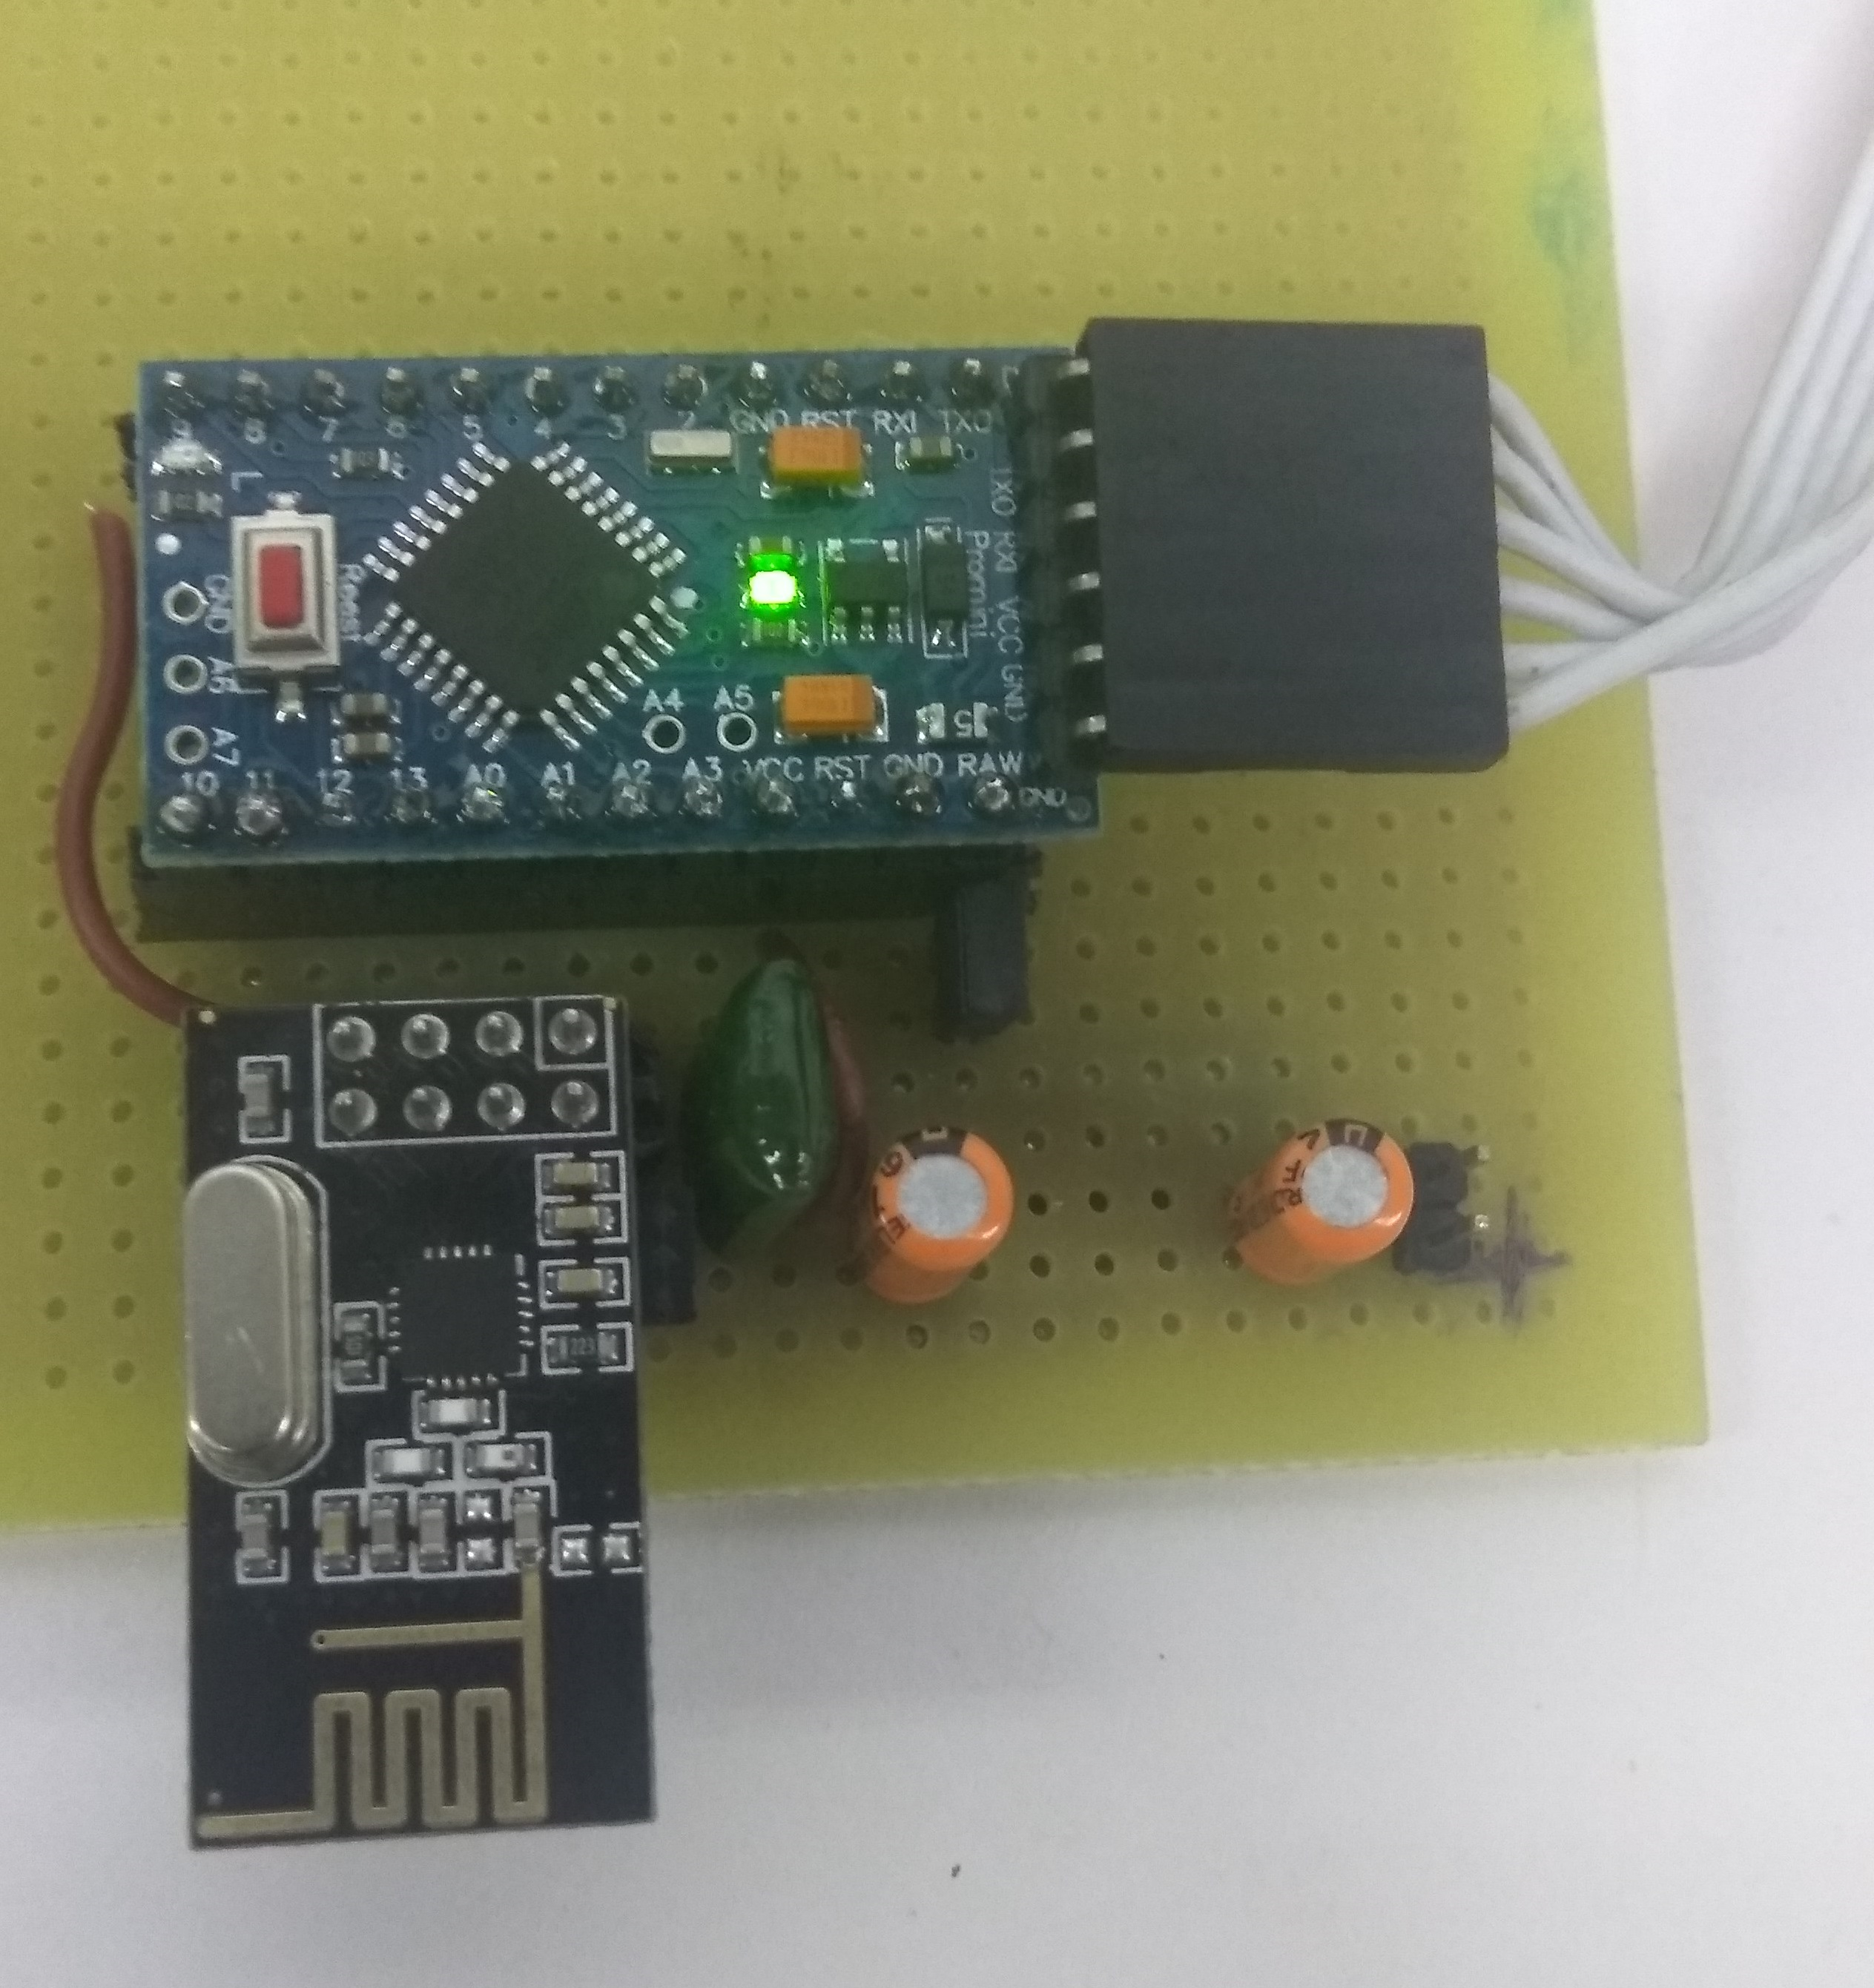
\includegraphics[width=0.5\textwidth]{IMG_20180605_144752.jpg}
\caption{Prototype Hardware}
\end{center}
\end{figure}

\end{frame}

\begin{frame}{Task Accomplished}
\begin{figure}
\begin{itemize}
\item PCB schematic design of final circuit
\end{itemize}
\begin{center}
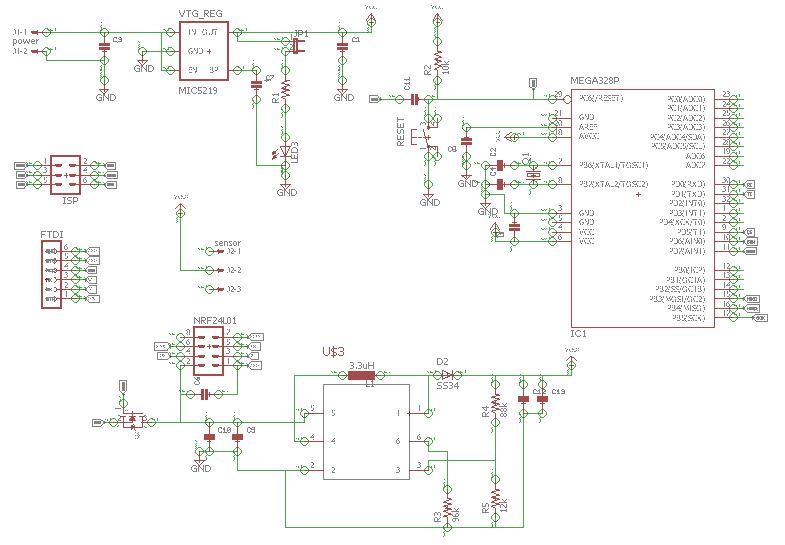
\includegraphics[width=0.85\textwidth]{Capture.JPG}
\caption{Schematic design of board}
\end{center}
\end{figure}
\end{frame}


\begin{frame}{Task Accomplished}
	\begin{itemize}
    \item Completed testing of star network by using two transmitter and one receiver
    \item Measure current of Arduino Pro Mini
    \begin{itemize}
    	\item Normal mode current = \textbf{11.5 mA} 
        \item Sleep mode current = \textbf{0.6 mA}
    \end{itemize}
    \item Measure current of nRF24L01
    \begin{itemize}
    	\item Normal mode current = \textbf{1.2 mA}  
        \item stand by mode current = \textbf{40 uA}
        \item Sleep mode current = \textbf{900 nA}
    \end{itemize}
    \item Test the range of nRF24L01 in outdoor environment with different data rate
    \begin{itemize}
    	\item  MIN (-18 dBm) power = \textbf{0 to 6 m}
        \item  LOW (-12 dBm) power = \textbf{0 to 8 m}
        \item  HIGH (-6 dBm) power = \textbf{0 to 12 m}
        \item  MAX (0 dBm) power = \textbf{0 to 16 m}
	\end{itemize}
    \end{itemize}
\end{frame}

\begin{frame}{Task Accomplished}
\begin{figure}
\begin{center}
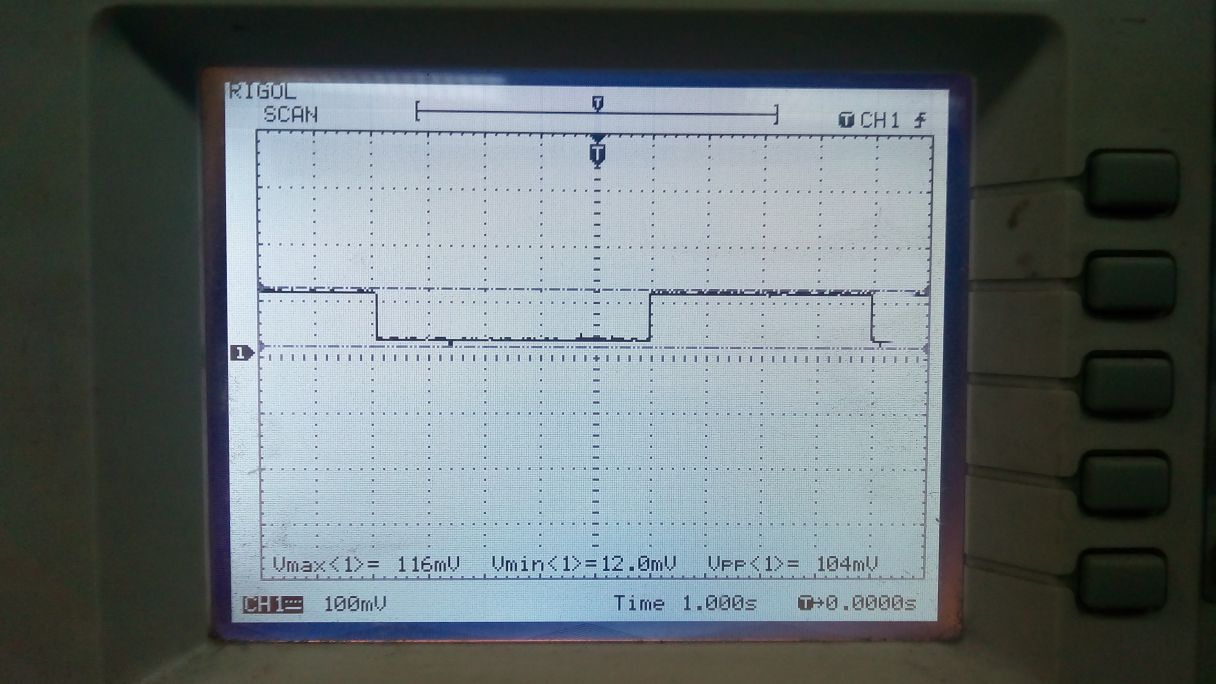
\includegraphics[width=1\textwidth]{pro_mini_current_vtg_2.jpeg}
\caption{Current of Arduino Pro Mini (Sleep mode, Idle mode)}
\end{center}
\end{figure}
\end{frame}

\begin{frame}{Task Accomplished}
\begin{figure}
\begin{center}

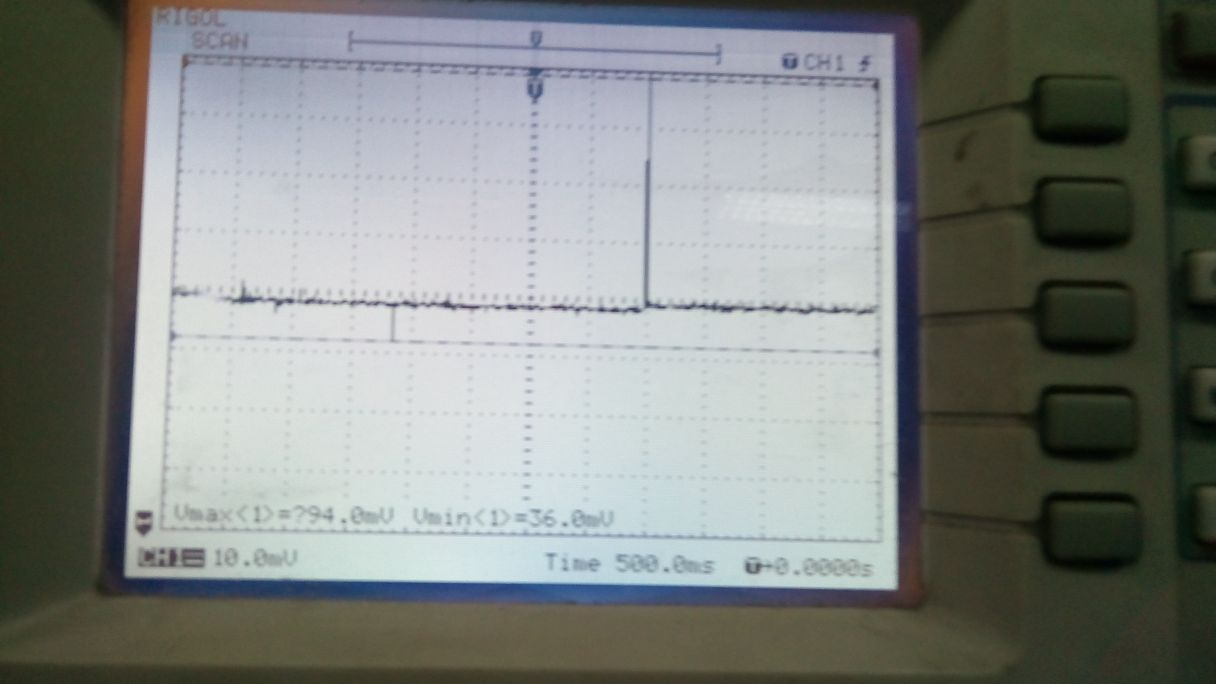
\includegraphics[width=1\textwidth]{IMG-20180606-WA0003.jpg}
\caption{Current of nRF24L01 (Active mode, Sleep mode)}
\end{center}
\end{figure}
\end{frame}
\begin{table}
\centering
  \caption{Range testing of nRF24L01 (At different data rates)}
    \begin{tabular}{|c|c|c|c|c|}
    \hline
    \multicolumn{1}{| p{5.715em} |}{Transmission \newline{}Power level} & \multicolumn{1}{ | p{3.715em} | }{MIN power\newline{}(-18 dBm)} & \multicolumn{1}{| p{4em} |}{LOW power\newline{}(-12 dBm)} & \multicolumn{1}{| p{4.145em} |}{HIGH power \newline{}(-6 dBm)} & \multicolumn{1}{|p{3.855em}|}{MAX power \newline{}(0 dBm)} \\
    \multicolumn{1}{|l|}{Distance (meter)} & & & & \\\hline
    3.8   & 100\% & 100\% & 100\% & 100\% \\\hline
    4.9   & 100\% & 100\% & 100\% & 100\% \\\hline
    5.9   & 100\% & 100\% & 100\% & 100\% \\\hline
    6.9   & 47\%  & 100\% & 100\% & 100\% \\\hline
    8     & 0\%   & 100\% & 100\% & 100\% \\\hline
    8.2   & 0\%   & 100\% & 100\% & 100\% \\\hline
    10    & 0\%   & 74\%  & 100\% & 100\% \\\hline
    12.4  & 0\%   & 0\%   & 100\% & 100\% \\\hline
    15.6  & 0\%   & 0\%   & 86\%  & 100\% \\\hline
    \end{tabular}
  \label{tab:addlabel}
\end{table}

\section{Challenges Faced}
\begin{frame}{Challenges Faced}
	\begin{itemize}
		\item Prototype testing of nRF24L01
        \item Range testing of nRF24L01 in outdoor environment
        \item Setting of fuse bits (Low, High, Extended) using AVRDude
        \item Importing RF24 library in Atmel Studio
        \item Differentiating data of two transmitter at one receiver
	\end{itemize} 
\end{frame}

\section{Future Plans}
\begin{frame}{Future Plans}
	\begin{itemize}
		\item PCB printing, soldering and testing
        \item Solve the problem of RF24 library in Atmel Studio, so that we can make example codes for prototype
        \item Duty cycling of ATmega328p
        \item Study about RF24mesh library
        \item Setup of 5 nodes WSN star network
        \item Use RPi as a gateway connected to master
        \item Operating life prediction of WSN
        \item Add soil moisture, light intensity sensor, humidity sensor on board and make provision to connect other sensors if needed
	\end{itemize}
\end{frame}


\section{Thank You}
\begin{frame}{Thank You}
	\centering THANK YOU !!!
\end{frame}
\end{document}
